\documentclass[handout]{beamer}

\usepackage{Haust2017glærur}

\title{Stærðfræðimynstur í tölvunarfræði}
\subtitle{Vika 2, seinni fyrirlestur}

\begin{document}

\begin{frame}
\titlepage
\end{frame}

\section{Inngangur}

\begin{frame}{Í síðasta tíma}
    \begin{itemize}
        \item Sannanir
        \begin{itemize}
            \item Beinar sannanir, sannanir með mótskilyrðingu, sannanir með mótsögn
        \end{itemize}
        \item Skoðuðum sýnidæmi í \LaTeX
    \end{itemize}
\end{frame}

\begin{frame}{Sókn í dæmahópa}
    Mjög ójöfn sókn í fyrstu dæmatímaviku.
    \begin{center}
        \begin{tabular}{lll}
            \toprule
            Hópur&Ástand\\
            \midrule
            d1 (fim. 11:40)&\emph{Of fjölmennt!}\\
            d2 (mið. 15:00)&Fámennt\\
            d3 (mið. 13:20 Lögberg)&Fámennt\\
            d4 (fim. 15:00 VRII)&Flott\\
            d5 (fim. 15:00 Árnagarður)&\emph{Of fámennt!}\\
            d6 (mið. 13:20 VRII)&Of fjölmennt\\
            d7 (fim. 13:20)& Of fjölmennt\\
            \bottomrule
        \end{tabular}
    \end{center}
    Endilega farið yfir Suðurgötuna og mætið seinna á daginn, getið fengið meiri þjónustu þannig.
\end{frame}

\section{Mengi og mengjaaðgerðir (2.1-2.2)}

\begin{frame}{Mengi}
\begin{itemize}
 \item Mengi (e. \emph{set}) er grundvallareining í strjálli stærðfræði
 \item Skyld hugmynd ``hópur'':
 \begin{itemize}
  \item Mengi eru notuð til að ``hópa'' hluti saman
  \item ``Hópur'' af hlutum myndar mengi
 \end{itemize}
 \item ``Hlutur'' í mengi er kallaður stak (e. \emph{member} eða \emph{element})
 \item Hlutir í sama mengi eiga oftast eitthvað sameiginlegt
 \item Dæmi um mengi: Allar heiltölur, allir nemendur í þessu námskeiði
\end{itemize}
\end{frame}

\begin{frame}{Skilgreining á mengi}

Klassísk skilgreining á mengi er eftirfarandi:
\begin{tcolorbox}[title=Mengi]
Mengi er óraðað samansafn hluta. Hlutur í mengi er kallaður stak þess. Mengi inniheldur stök sín. $a \in A$ táknar að stakið $a$ sé í menginu $A$. $a \notin A$ táknar að $a$ sé ekki í $A$.
\end{tcolorbox}

\end{frame}

\begin{frame}{Að tilgreina mengi}
\begin{itemize}
 \item Slaufusvigar eru oftast notaðir til að afmarka mengi
 \item Nokkrar leiðir eru algengar þegar kemur að því að tilgreina stök mengis
 \begin{itemize}
  \item Að telja upp öll stökin: 
  \begin{itemize}
   \item Mengi enskra sérhljóða: $\{a, e, i, o, u\}$
  \end{itemize}
  \item Að sýna mynstur og láta þrípunkt tákna ``augljósa'' endurtekningu:
  \begin{itemize}
   \item Mengi jákvæðra heiltalna minni en 100: $\{1, 2, 3,\ldots, 100\}$
  \end{itemize}
  \item Að tilgreina skilyrði sem stök þurfa að uppfylla (e. \emph{set builder notation}):
  \begin{itemize}
   \item $\{x \in \mathbf{Z^+} | x < 100\}$
  \end{itemize}
 \end{itemize}
 \item Sum mengi hafa stöðluð nöfn: $\mathbf{R}$ (mengi rauntalna), $\mathbf{Z^+}$ (mengi jákvæðra heiltalna), \ldots
\end{itemize}
\end{frame}

\begin{frame}{Hvað má fara í mengi?}
\begin{itemize}
 \item Skilgreiningin okkar á mengjum leyfir ýmislegt
 \begin{itemize}
  \item Mengi af mengjum: $\{\mathbf{N}, \mathbf{Z}, \mathbf{Q}, \mathbf{R}\}$
 \end{itemize}
 \item Tómt mengi, táknað $\emptyset$
 \begin{itemize}
  \item Mengi sem inniheldur tóma mengið $\{\emptyset\}$
 \end{itemize}
 \item Þessi opna skilgreining veldur tæknilegum vandræðum
\end{itemize}
\end{frame}

\begin{frame}{Vandræði}
\begin{itemize}
 \item Látum $S$ vera mengið sem inniheldur þau mengi $x$ sem ekki innihalda sig sjálf, þ.e.a.s.
\end{itemize}
\[
 S = \{x | x \notin x\}
\]
\begin{itemize}
 \item Er $S$ í sjálfu sér? \pause
 \begin{itemize}
  \item Ef já, þá verður það að uppfylla það skilyrði að vera ekki í sjálfu sér \pause
  \item Ef nei, þá uppfyllir það skilyrðið sem það þarf að uppfylla til að vera í sjálfu sér \pause
 \end{itemize}
 \item Þversögn. Leiddi til frumsendulegrar mengjafræði (e. \emph{axiomatic set theory}), sem er strangari
 \begin{itemize}
  \item Þversögnin er kennd við Russell, (e. \emph{Russell's Paradox})
 \end{itemize}

\end{itemize}
\end{frame}

\begin{frame}{Jöfn mengi}
\begin{tcolorbox}[title=Jöfn mengi]
Tvö mengi eru jöfn (e. \emph{equal}) ef þau innihalda sömu stök, þ.e.a.s. $\forall x (x \in A \leftrightarrow x \in B ) $. Við skrifum $A = B$ ef mengin $A$ og $B$ eru jöfn.
\end{tcolorbox}
Til dæmis eru mengin $\{a, b, c\}$ og $\{b, c, a\}$ jöfn. Sömuleiðis $\{a, b, c\}$ og $\{a, a, b, c\}$.
\end{frame}

\begin{frame}{Hlutmengi}
\begin{tcolorbox}[title=Hlutmengi]
Mengið $A$ er hlutmengi í (e. \emph{subset of}) $B$ þá og því aðeins að hvert stak í $A$ sé einnig í $B$, þ.e.a.s. $\forall x (x \in A \to x \in B)$. Við skrifum $A \subseteq B$ ef $A$ er hlutmengi í $B$.
\end{tcolorbox}

Athugum að séu tvö mengi jöfn, þá er $A \subseteq B$ og $B \subseteq A$.
\end{frame}

\begin{frame}{Tóma mengið sem hlutmengi}
\begin{itemize}
 \item Er tóma mengið hlutmengi í öllum mengjum? \pause
 \item Athugum skilgreininguna:
 \begin{itemize}
  \item Látum $S$ vera mengi. Gildir $\forall x (x \in \emptyset \to x \in S)$? \pause
  \item $x \in \emptyset$ er alltaf ósatt \pause
  \item $p \to q$ er alltaf satt þegar $p$ er ósatt
 \end{itemize}
\end{itemize}
\end{frame}

\begin{frame}{Fjöldatala mengis}
\begin{tcolorbox}[title=Fjöldatala]
Látum $S$ vera mengi. Séu $n$ mismunandi stök í $S$ og $n \in \mathbf{Z^+}$, þá er $S$ endanlegt mengi (e. \emph{finite set}) og $n$ er fjöldatala (e. \emph{cardinality}) mengisins $S$. Fjöldatala (eða stærð) mengisins $S$ er táknuð með $|S|$.
\end{tcolorbox}
Hægt er að skilgreina fjöldatölur fyrir mengi sem eru ekki endanleg.
\end{frame}

\begin{frame}{Veldismengi mengis}
\begin{tcolorbox}[title=Veldismengi]
Látum $S$ vera mengi. Þá er veldismengi (e. \emph{power set}) $S$ mengi allra hlutmengja $S$. Veldismengi $S$ er táknað með $\mathbf{P}(S)$.
\end{tcolorbox}
Dæmi: \[\mathbf{P}(\{0, 1\}) = \pause \{\emptyset, \{0\}, \{1\}, \{0, 1\}\}\]

Athugum að tóma mengið og mengið sjálft eru alltaf stök í veldismengi mengis.
\end{frame}

\begin{frame}{Mengjamargfeldi}
\begin{tcolorbox}[title=Mengjamargfeldi]
Látum $A$ og $B$ vera mengi. Mengjamargfeldi (e. \emph{cartesian product}) $A$ og $B$ er mengi allra raðaðra para $(a, b)$ þar sem $a \in A$ og $b \in B$, þ.e.a.s. mengið $\{(a, b) | a \in A \land b \in B\}$. Mengjamargfeldi $A$ og $B$ er táknað með $A \times B$.
\end{tcolorbox}
Dæmi:
\[
 \{1, 2\} \times \{a, b\} = \pause \{(1, a), (1, b), (2, a), (2, b)\}
\]
Athugum að almennt gildir ekki að $A \times B$ sé jafnt $B \times A$.
\end{frame}

\begin{frame}{Sannmengi}
    Við getum tengt saman hugmyndir úr umsagnarökfræði og mengjafræði
    \begin{tcolorbox}[title=Sannmengi]
        Látum $P$ vera umsögn og $D$ vera óðal. Sannmengi (e. \emph{truth set}) $P$ er mengi þeirra staka $x$ í $D$ sem gerir $P(x)$ satt, þ.e.a.s.

        \[
            \{x \in D | P(x)\}
        \]
    \end{tcolorbox}

    Dæmi: Sannmengi $P(x) = '|x| = 1'$ þar sem óðalið er mengi heiltalna er mengið $\{x \in \mathbf{Z} | |x|=1\} = $\pause $\{-1,1\}$
\end{frame}

\begin{frame}{Sammengi}
\begin{tcolorbox}[title=Sammengi]
Látum $A$ og $B$ vera mengi. 
Sammengi (e. \emph{union}) mengjanna er mengið sem inniheldur stökin sem eru í $A$ eða $B$, 
þ.e.a.s. mengið $\{x | x \in A \lor x \in B \}$. 
Sammengi $A$ og $B$ er táknað með $A\cup B$.
\end{tcolorbox}
Dæmi:
\[
 \{1, 3\} \cup \{1, 2, 4\} = \pause \{1, 2, 3, 4\}
\]
\end{frame}

\begin{frame}{Sniðmengi}
\begin{tcolorbox}[title=Sniðmengi]
Látum $A$ og $B$ vera mengi.
Sniðmengi (e. \emph{intersection}) mengjanna er mengið sem inniheldur stökin sem eru í $A$ og $B$, 
þ.e.a.s. mengið $\{x | x \in A \land x \in B \}$. 
Sniðmengi $A$ og $B$ er táknað með $A\cap B$.
\end{tcolorbox}
Mengi eru kölluð sundurlæg (e. \emph{disjoint}) ef sniðmengi þeirra er tóma mengið.

Dæmi um sniðmengi:
\[
 \{1, 3\} \cap \{1, 2, 4\} = \pause \{1\}
\]
\end{frame}

\begin{frame}{Mengjamismunur}
\begin{tcolorbox}[title=Mengjamismunur]
Mismunur mengjanna $A$ og $B$ er mengi þeirra staka sem eru í $A$ en ekki í $B$, þ.e.a.s. mengið $\{x | x \in A \land x \notin B\}$.
\end{tcolorbox}
Mengjamismunur $A$ og $B$ er táknaður með $A - B$ í bókinni. Aðrar bækur nota ritháttinn $A \setminus B$.
\end{frame}

\begin{frame}{Almengi og fyllimengi}
Fyrir mengi er hægt að skilgreina mengi allra mögulegra staka, kallað almengi (e. \emph{universal set}) oft táknað með $U$. Þá má skilgreina:

\begin{tcolorbox}[title=Fyllimengi]
Látum $A$ vera mengi og $U$ almengi þess. Þá er fyllimengi $A$ m.t.t. $U$ mengið $U - A$. Fyllimengi $A$ er táknað með $\overline{A}$.
\end{tcolorbox}

Algengt er að nefnd mengi á borð við $\mathbf{R}$ eða $\mathbf{N}$ þjóni sem almengi.
\end{frame}

\begin{frame}{Mengjajafngildi}
\begin{columns}
\column{0.3\textwidth}
Með þessum skilgreiningum má rökstyðja ýmis jafngildi fyrir mengi.

\vspace*{0.5cm}
Tafla úr kafla 2.2.
\column{0.7\textwidth}
\begin{center}
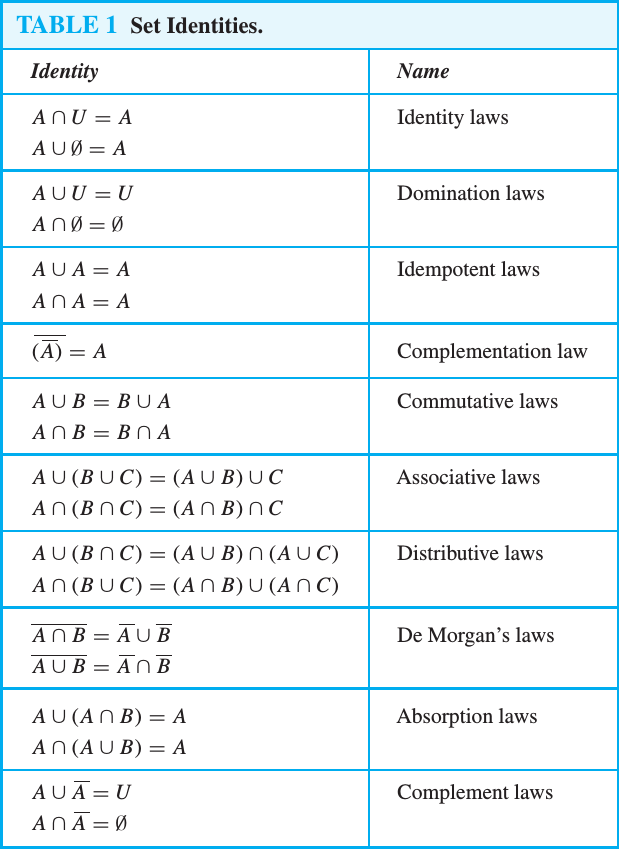
\includegraphics[height=0.8\textheight]{set-equivalences}
\end{center}
\end{columns}
\end{frame}

\begin{frame}{Útleiðsla á De Morgan fyrir mengi}
Viljum sýna að $\overline{A \cap B} = \overline{A} \cup \overline{B}$. \pause

\begin{align*}
\overline{A \cap B} &= \{x | x \notin A \cap B\}\\ 
&= \{x | \lnot ( x \in A \cap B)\}\\ 
&= \{x | \lnot ( x \in A \land x \in B)\}\\ 
&= \{x | \lnot ( x \in A) \lor \lnot (x \in B)\}\\ 
&= \{x | x \notin A \lor x \notin B\}\\ 
&= \{x | x \in \overline{A} \lor x \in \overline{B}\}\\ 
&= \{x | x \in \overline{A} \cup \overline{B}\}\\ 
&= \overline{A} \cup \overline{B}
\end{align*}
\end{frame}

\begin{frame}{Meðlimatöflur}
Hægt er að kanna jafngildi með meðlimatöflu, sem svipar til sanntöflu:
\begin{center}
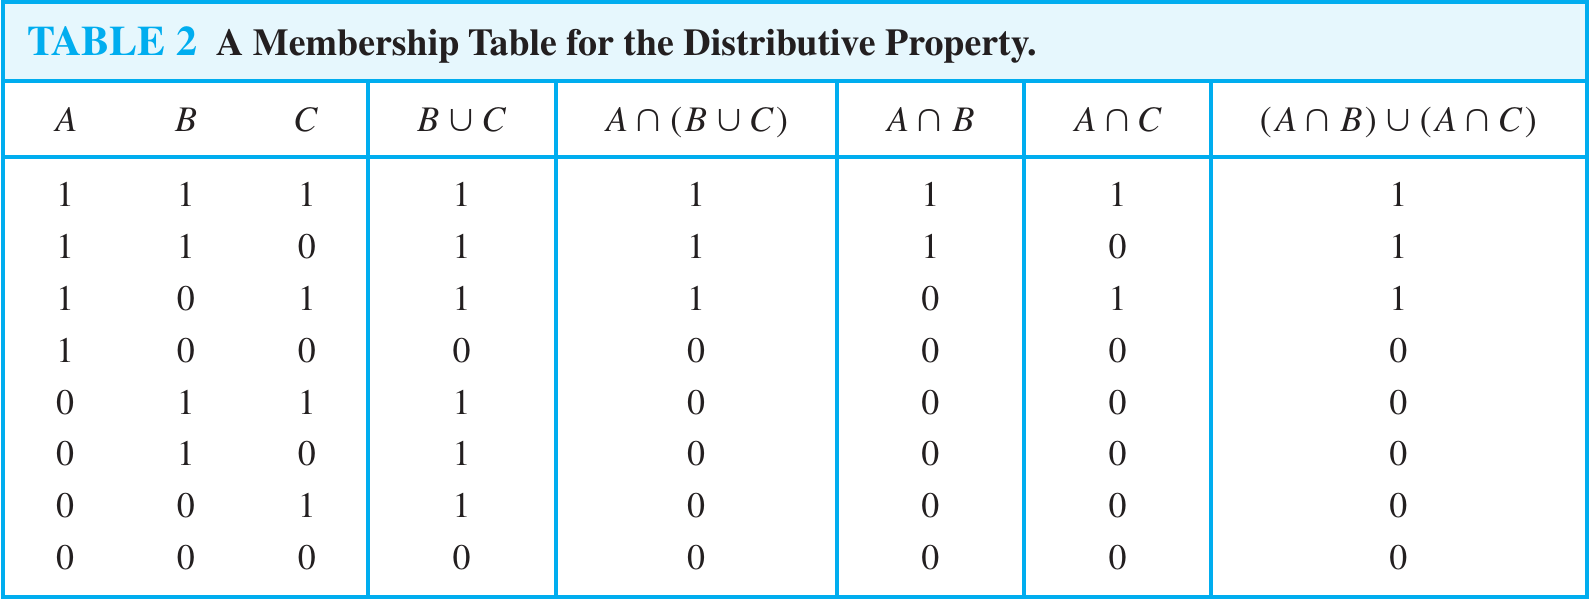
\includegraphics[width=\textwidth]{membership-table}
\end{center}
\end{frame}

\begin{frame}{Útvíkkun}
Sammengi margra mengja er mengi þeirra staka sem er í a.m.k. einu mengjanna:
\[
 A_1 \cup A_2 \cup \ldots \cup A_n = \bigcup_{i=1}^n A_i
\]
Sniðmengi margra mengja er mengi þeirra staka sem er í öllum mengjunum:
\[
 B_1 \cap B_2 \cap \ldots \cap B_n = \bigcap_{i=1}^n B_i
\]
\end{frame}

\section{Mengi í tölvum}

\begin{frame}[fragile]{Gagnagerðir sem mengi}
 \begin{itemize}
  \item Hugmyndin um gagnagerð (e. \emph{data type}) byggir á mengjum
  \item Gagnagerð samanstendur af mengi mögulegra gilda og aðgerðum á þau
  \item Gagnagerðin \texttt{Boolean} í Java skilgreinist af:
  \begin{itemize}
   \item Menginu \{\texttt{true},\texttt{false}\}
   \item Aðgerðum: Og (\verb|&&|), eða (\verb&||&), \ldots
  \end{itemize}
 \end{itemize}
\end{frame}

\section{Föll}

\begin{frame}{Föll}
\begin{itemize}
 \item Fall er hugtak sem er mörgum kunnuglegt úr stærðfræðigreiningu
 \begin{itemize}
  \item $f(x) = x^2$ er fall
  \item $\sin(x)$ er fall
 \end{itemize}
 \item Oftast hefur verið um að ræða föll sem taka inn eina rauntölu og skila annarri rauntölu
 \begin{itemize}
  \item Við notum opnari skilgreiningu
 \end{itemize}
\end{itemize}
\end{frame}

\begin{frame}{Skilgreining á falli}
\begin{tcolorbox}[title=Fall]
Látum $A$ og $B$ vera mengi sem eru ekki tóm. Fall (e. \emph{function}) $f$ frá $A$ til $B$ er ákvörðun á nákvæmlega einu staki í $B$ fyrir sérhvert stak í $A$.

Við skrifum $f(a) = b$ þegar $b$ er stakið sem fallið $f$ ákvarðar fyrir stakið $a$.

Við skrifum $f: A \to B$ þegar $f$ er fall frá $A$ til $B$.
\end{tcolorbox}

Föll eru líka kölluð varpanir (e. \emph{mapping} eða \emph{transformation}). Fall $f: A \to B$ varpar stökum úr mengi $A$ yfir í mengi $B$.
\end{frame}

\begin{frame}{Dæmi um föll}
\begin{itemize}
 \item Föll sem skilgreind eru með formúlu, föll með þekkt nöfn
 \begin{itemize}
  \item $f(x) = x^2$ er $\mathbf{R} \to \mathbf{R}$
  \item $\sin(x)$ er líka $\mathbf{R} \to \mathbf{R}$
 \end{itemize}
 \item Ákvörðun einkunna í þessu námskeiði má tákna með falli
 \item Ákvörðun nafna út frá kennitölum má tákna með falli \pause
 \begin{itemize}
  \item Ákvörðun kennitalna út frá nöfnum er ekki fall!
 \end{itemize}
\end{itemize}
\end{frame}

\begin{frame}{Formengi og bakmengi}
\begin{tcolorbox}[title=Formengi og bakmengi]
Sé $f$ fall frá $A$ til $B$ kallast $A$ formengi (e. \emph{domain}) fallsins og $B$ bakmengi (e. \emph{codomain}) þess. Sé $f(a) = b$ er sagt að $b$ sé mynd (e. \emph{image}) $a$ og að $a$ sé formynd (e. \emph{preimage}) $a$.
\end{tcolorbox}
Sum föll eru hlutskilgreind (e. \emph{partial functions}), þ.e.a.s. að þau eru ekki skilgreind fyrir öll stök í formengi sínu. Dæmi: $f(x) = 1/x$.
\end{frame}

\begin{frame}[fragile]{Föll í forritun}
\begin{itemize}
 \item Föll eru gríðarlega mikið notuð í forritun, í ýmsum myndum
 \begin{itemize}
  \item Dæmigert fall í forritun:
  \begin{itemize}
   \item Tekur inn breytur
   \item Framkvæmir reikniaðgerðir
   \item Skilar niðurstöðu í samræmi við inntakið 
  \end{itemize}
 \end{itemize}
 \item Í mörgum forritunarmálum eru formengi og bakmengi tilgreind þegar fall er skilgreint
\end{itemize}
\begin{minted}[frame=lines]{java}
// Fall frá mengi strengja til mengi heiltalna
static int f (String s) {
  ...
}
\end{minted}

\end{frame}

\begin{frame}{Eintæk föll}
\begin{tcolorbox}[title=Eintækt fall]
Fall er eintækt (e. \emph{injective} eða \emph{one-to-one}) ef það varpar engum tveimur stökum í formengi sínu í sama stak bakmengisins, þ.e.a.s. ef \[\forall a \forall b ((f(a) = f(b)) \to (a = b))\] og þar með \[\forall a \forall b ((a \neq b) \to (f(a) \neq f(b)))\].
\end{tcolorbox}

Er fallið $f: \mathbf{R} \to \mathbf{R}$, $f(x) = x + 1$ eintækt? \pause

Já, athugum að sé $x \neq y$, þá $x + 1 \neq y + 1$.
\end{frame}

\begin{frame}{Átæk föll}
\begin{tcolorbox}[title=Átækt fall]
Fall $f$ er átækt (e. \emph{surjective} eða \emph{onto}) ef það ``þekur'' bakmengi sitt, þ.e.a.s. að fyrir hvert stak $b$ í bakmenginu er til stak í formenginu $a$ svo að $f(a) = b$, \[\forall b \exists a (f(a) = b)\].
\end{tcolorbox}
Er fallið $f: \mathbf{Z} \to \mathbf{Z}$, $f(x) = x^2$ átækt? \pause

Nei, engin heiltala gefur $f(x) = -1$, til dæmis.
\end{frame}

\begin{frame}{Eintækni og átækni}
\begin{center}
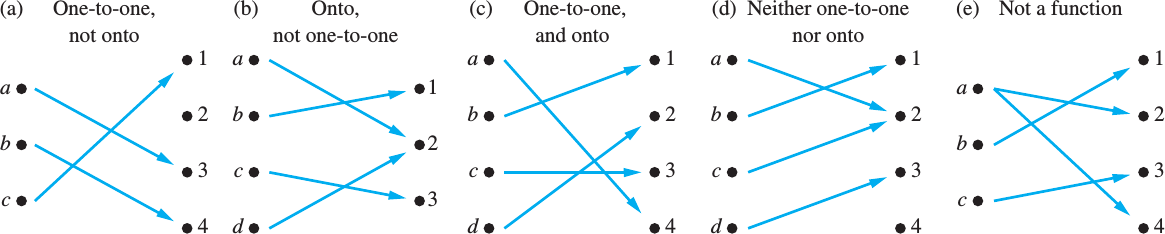
\includegraphics[width=\textwidth]{function-types}
\end{center}
Fall sem er bæði eintækt og átækt er kallað gagntækt (e. \emph{bijective}).
\end{frame}

\begin{frame}{Andhverfanleg föll}
\begin{tcolorbox}[title=Andhverfanlegt fall]
Látum $f$ vera gagntækt fall frá $A$ til $B$. Þá er andhverfa fallsins $f$ fallið sem varpar $b \in B$ í stakið $a \in A$ sem um gildir að $f(a) = b$.

Andhverfa fallsins $f$ er táknuð með $f^{-1}$. Um $f^{-1}$ gildir:

\[
 f(a) = b \equiv f^{-1}(b) = a
\]

\end{tcolorbox}
Fall sem er ekki gagntækt er óandhverfanlegt. Hægt er að búa til andhverfanlegt fall úr óandhverfanlegu með því að takmarka formengi þess.
\end{frame}

\begin{frame}{Samantekt}
\begin{itemize}
 \item Látum $f: A \to B$
 \begin{itemize}
  \item Til að sýna að fall sé eintækt: Sýna að sé $f(x) = f(y)$ fyrir ótilgreind $x, y \in A$, þá sé $x = y$.
  \item Til að sýna að fall sé átækt: Athuga ótilgreint $y \in B$ og finna $x \in A$ svo að $f(x) = y$
 \end{itemize}
 \item Til að sýna fram á hið gagnstæða, finnið mótdæmi
\end{itemize}

\end{frame}


\begin{frame}{Samskeyting falla}
\begin{tcolorbox}[title=Samskeyting falla]
Látum $g$ vera fall frá menginu $A$ til mengisins $B$ og látum $f$ vera fall frá menginu $B$ til mengisins $C$. Samskeyting (e. \emph{composition}) fallanna $f$ og $g$, fyrir $a \in A$ er þá táknuð með $f \circ g$ og skilgreinist af

\[
 (f \circ g)(a) = f(g(a))
\]

\end{tcolorbox}
Oft er hægt að einfalda föll með því að skrifa þau sem samskeytingar. Við forritun kemur þetta sérstaklega við í fallsforritunarmálum.
\end{frame}

\begin{frame}{Næst}
Runur og rakningarvensl (kafli 2.4), reiknanleiki (kafli 2.5), fylki (kafli 2.6)
\end{frame}


\end{document}
